\newpage

\subsection{Radian measure}


\begin{theorybox}{}

A radian is a unit of measure of angles. It is the constant angle that is formed at the centre of a circle when the arc length is equal to the radius.
\begin{center}
    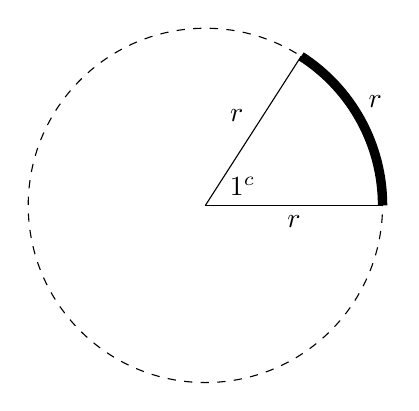
\begin{tikzpicture}[scale=0.75]
        \draw[dashed] (0,0) circle (3cm);
        \draw[line width=1.2mm] (3,0) arc[start angle=0, end angle=57.2958,radius=3cm];
        \draw (0,0) -- node[below]{$r$} (3,0);
        \draw (0,0) -- node[above left]{$r$} (1.6209,2.5244);
        \coordinate[label=above right: $r$] (P) at (2.5981, 1.5);
        \coordinate[label=above right: $1^{c}$] (O) at (0.25,0);
    \end{tikzpicture}
\end{center}

Compare this sector to an equilateral triangle whose angles are all $60^{\circ}$.

\begin{center}
    \begin{tikzpicture}[scale=0.75]
        \draw[dashed, blue] (0,0) -- (5,0) -- (2.5, 4.3301) -- cycle;
        \draw[dotted, red,thick] (0,0) -- (5,0);
        \draw[dotted, red, thick] (2.7015, 4.2073) -- (0,0);
        \draw[thick, red, dotted] (5,0) arc[start angle=0, end angle=57.2958,radius=5cm];
        
    \end{tikzpicture}
\end{center}

We can see that $1^{c}$ is less than $60^{\circ}$. More accurately, $$1^{c} \approx 57.2958^{\circ}$$



Arranging three equilateral triangles, we can form one long straight edge.
\begin{center}
    \begin{tikzpicture}[scale=0.75]
        \draw[dashed, ] (0,0) -- (5,0) -- (2.5, 4.3301) -- cycle;
        \draw[dashed, ] (2.5, 4.3301)  -- (7.5, 4.3301) -- (5,0);
        \draw[dashed, ] (7.5, 4.3301) -- (10,0) -- (5,0) ;
        \draw [thick] (0,0) -- (10,0);
    \end{tikzpicture}
\end{center}

This is not the case when using the sectors with central angle $1^{c}$.
\begin{center}
    \begin{tikzpicture}[scale=0.75]
        \draw[dashed, ] (10,0) arc[start angle=0, end angle=57.2958,radius=5cm] -- (5,0);
        \draw[dashed, ] (7.70151,4.20735) arc[start angle=57.2958, end angle=114.5916,radius=5cm] -- (5,0);
        \draw[dashed, ] (2.9193,4.546487) arc[start angle=114.5916, end angle=171.8874,radius=5cm] -- (5,0);

        \draw [thick] (0,0) -- (10,0);
    \end{tikzpicture}
\end{center}

\clearpage

From the previous diagram, we can see that it takes a little bit more than $3^{\circ}$ to form $180^{\circ}$.
\vskip3mm
In fact, $180^{\circ} - 3 \times 57.2958^{\circ} \approx 8.1126^{\circ}$ remains.
\vskip3mm
$$\dfrac{8.1126}{57.2958} \approx 0.1415915 \dots$$
Hence, 
\begin{align*}
    3+0.1415915\dots \,  \text{radians} &=180^{\circ}   \\
    \therefore \pi \ \text{radians} &= 180^{\circ} 
\end{align*}

In practice, we do not write \textit{`radians'} so we often see $$\pi \cancel{\text{ radians}} = 180^{\circ}$$

The diagram below summarises the relationship between degrees and radians

\begin{center}
\begin{tikzpicture}
    \node [] (A)              {Degrees};
    \node [] (B) [right=of A] {Radians};
    
    \draw [thick, ->]
    (A) edge [bend left=45] node[above]{$\times \dfrac{\pi}{180}$} (B)
    (B) edge [bend left=45] node[below]{$\times \dfrac{180}{\pi}$} (A);
    
\end{tikzpicture}
\end{center}


\end{theorybox}

\vspace{5mm}

\begin{examplecz}[height fill=true]{}
    Express the following angles in radians, leaving your answer in terms of $\pi$.
    \begin{enumerate}
    \begin{multicols}{3}
        \item $360^{\circ}$
        \item $270^{\circ}$
        %\item $180^{\circ}$
        \item $120^{\circ}$
        \item $90^{\circ}$
        \item $45^{\circ}$
        %\item $60^{\circ}$
        %\item $30^{\circ}$
        \item $540^{\circ}$
    \end{multicols}
    \end{enumerate}
\tcblower
\textbf{Solution:}
%\vspace*{cm}
\end{examplecz}

\begin{examplecz}{}
    Express the following angles in radians, correct to three decimal places.
    \begin{enumerate}
    \begin{multicols}{3}
        \item $360^{\circ}$
        %\item $270^{\circ}$
        %\item $180^{\circ}$
        %\item $120^{\circ}$
        %\item $150^{\circ}$
        %\item $400^{\circ}$
        %\item $210^{\circ}$
        %\item $105^{\circ}$
        %\item $315^{\circ}$
        \item $17^{\circ}$
        \item $62.8^{\circ}$
    \end{multicols}
    \end{enumerate}
\tcblower
\textbf{Solution:}
\vspace{60mm}
\end{examplecz}

\vspace{5mm}

\begin{examplecz}{}
    Express the following angles in degrees, to the nearest minute.
    \begin{enumerate}
    \begin{multicols}{3}
        \item $\dfrac{5 \pi}{4}$
        \item $0.6$
        \item $\dfrac{4 \pi}{5}$
        \item $\dfrac{3 \pi}{2}$
        \item $4.35$
        \item $\dfrac{ \pi}{6}$
        %\item $\dfrac{ \pi}{3}$
        %\item $\dfrac{3}{10}$
        %\item $1.6$
        
    \end{multicols}
    \end{enumerate}
\tcblower
\textbf{Solution:}
\vspace{60mm}
\end{examplecz}

\vfill

\begin{Qbox}{}
    From \textit{CambridgeMaths Year 11 Mathematics Extension 1}:
    \begin{itemize}
        \item Exercise 11G: 1 to 8, 11
    \end{itemize}
\end{Qbox}